% Thesis Figure 6.2: placement of the autoencoder in the partner VGG16 classifier, redrawn
% after D7.2 Figures 13 and 11 (p. 14); the originals stay in ../sparta/report-originals/.
% D7.2 Section 2.3.2.3.2: the initial autoencoder is trained on the dataset and inserted
% before the CNN; the middle autoencoder is trained on VGG16 outputs and inserted before the
% DNN; in both, VGG16 and the DNN keep their original weights. D7.6 p. 29 names the two
% versions top and middle, as the chapter and its benchmark table do. Symbols follow
% Equation eq:advml:compositions: r_{eta_x} and r_{eta_z} the autoencoders, phi_omega the
% feature extractor and c_psi the prediction head.
% lmodern is loaded before the shared style so that math scales to the small sizes used
% here; the style then sets the text face to TeX Gyre Heros as in the other figures.
% Geometry is in millimetres with y pointing down; 140 mm fits the text block at 1:1.
\documentclass[border=1pt]{standalone}
\usepackage{lmodern}
% Shared typography and palette for the three corrected SWaT context figures.
% Geometry is in millimetres; 140 mm fits the thesis text block at native scale.
\usepackage[T1]{fontenc}
\usepackage{tgheros}
\renewcommand{\familydefault}{\sfdefault}
\usepackage{tikz}
\usetikzlibrary{calc,patterns}
\definecolor{swatblue}{HTML}{0065BD}
\definecolor{swatlight}{HTML}{98C6EA}
\definecolor{swatgrey}{HTML}{666666}
\tikzset{every node/.style={font=\fontsize{8}{10}\selectfont},
  panel/.style={draw=black!30,fill=white,line width=0.4pt},
  stage/.style={draw=swatblue,fill=swatblue,text=white,align=center,
    minimum height=10mm,text width=19mm,inner sep=0.5mm},
  smalllabel/.style={font=\fontsize{7}{8.5}\selectfont,text=swatgrey}}

\usetikzlibrary{arrows.meta}
\newcommand{\fT}{\fontsize{7.5}{9}\selectfont\bfseries}
\newcommand{\fH}{\fontsize{7}{8.4}\selectfont\bfseries}
\newcommand{\fB}{\fontsize{7}{8.4}\selectfont\mdseries}
\newcommand{\fS}{\fontsize{6.5}{7.8}\selectfont\mdseries}
% Stages. #1 left x, #2 right x, #3 centre y.
\newcommand{\inbox}[3]{%
  \draw[op] (#1,{#3-4}) rectangle (#2,{#3+4});
  \node[txt] at ({(#1+#2)/2},#3) {\fB Input data};}
\newcommand{\outbox}[3]{%
  \draw[outbox] (#1,{#3-4}) rectangle (#2,{#3+4});
  \node[txt] at ({(#1+#2)/2},#3) {\fH Prediction};}
% Trapezoid narrowing along the flow: #4 left and #5 right half-height, #6 label.
\newcommand{\trap}[6]{%
  \draw[netout] (#1,{#3-#4}) -- (#2,{#3-#5}) -- (#2,{#3+#5}) -- (#1,{#3+#4}) -- cycle;
  \node[txt,text=swatblue] at ({(#1+#2)/2},#3) {\fH #6};}
% Autoencoder: encoder narrowing to a code, decoder widening back.
\newcommand{\autoenc}[3]{%
  \pgfmathsetmacro{\xm}{(#1+#2)/2}%
  \fill[swatblue] (#1,{#3-6}) -- (\xm,{#3-1.6}) -- (#2,{#3-6})
    -- (#2,{#3+6}) -- (\xm,{#3+1.6}) -- (#1,{#3+6}) -- cycle;
  \draw[white,line width=0.5pt] (\xm,{#3-1.6}) -- (\xm,{#3+1.6});}
% Label under a stage, on a common baseline: centre x, centre y of the stage, colour, text.
\newcommand{\under}[4]{\node[txt,anchor=base,text=#3] at (#1,{#2+9.3}) {\fS #4};}
\begin{document}
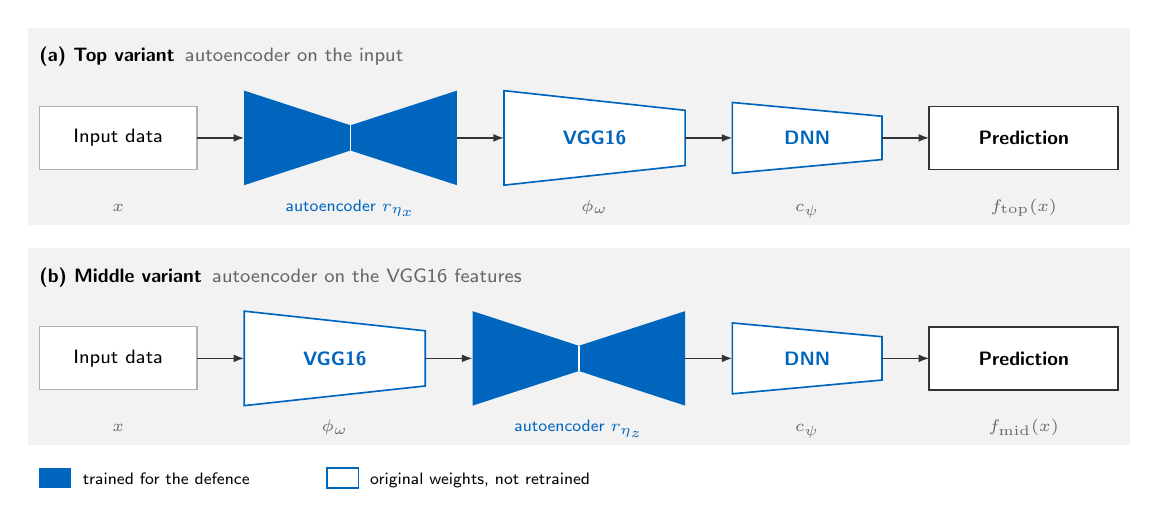
\begin{tikzpicture}[x=1mm,y=-1mm,
    txt/.style={inner sep=0pt,outer sep=0pt},
    op/.style={draw=black!30,fill=white,line width=0.4pt},
    netout/.style={draw=swatblue,fill=white,line width=0.6pt},
    outbox/.style={draw=black!80,fill=white,line width=0.6pt},
    lnk/.style={draw=black!80,line width=0.6pt},
    arr/.style={lnk,-{Latex[length=1.35mm,width=1mm]}}]
  \path[use as bounding box] (0,0) rectangle (140,60);

  % (a) Top variant: autoencoder on the input
  \fill[black!5] (0,0) rectangle (140,25);
  \node[txt,anchor=base west] at (1.5,4.3)
    {\fT (a) Top variant\hspace{1.3mm}{\fB\color{swatgrey}autoencoder on the input}};
  \inbox{1.5}{21.5}{14}
  \autoenc{27.5}{54.5}{14}
  \trap{60.5}{83.5}{14}{6}{3.5}{VGG16}
  \trap{89.5}{108.5}{14}{4.5}{2.75}{DNN}
  \outbox{114.5}{138.5}{14}
  \draw[arr] (21.5,14) -- (27.5,14);
  \draw[arr] (54.5,14) -- (60.5,14);
  \draw[arr] (83.5,14) -- (89.5,14);
  \draw[arr] (108.5,14) -- (114.5,14);
  \under{11.5}{14}{swatgrey}{$x$}
  \under{41}{14}{swatblue}{autoencoder $r_{\eta_x}$}
  \under{72}{14}{swatgrey}{$\phi_\omega$}
  \under{99}{14}{swatgrey}{$c_\psi$}
  \under{126.5}{14}{swatgrey}{$f_{\mathrm{top}}(x)$}

  % (b) Middle variant: autoencoder on the VGG16 features
  \fill[black!5] (0,28) rectangle (140,53);
  \node[txt,anchor=base west] at (1.5,32.3)
    {\fT (b) Middle variant\hspace{1.3mm}{\fB\color{swatgrey}autoencoder on the VGG16 features}};
  \inbox{1.5}{21.5}{42}
  \trap{27.5}{50.5}{42}{6}{3.5}{VGG16}
  \autoenc{56.5}{83.5}{42}
  \trap{89.5}{108.5}{42}{4.5}{2.75}{DNN}
  \outbox{114.5}{138.5}{42}
  \draw[arr] (21.5,42) -- (27.5,42);
  \draw[arr] (50.5,42) -- (56.5,42);
  \draw[arr] (83.5,42) -- (89.5,42);
  \draw[arr] (108.5,42) -- (114.5,42);
  \under{11.5}{42}{swatgrey}{$x$}
  \under{39}{42}{swatgrey}{$\phi_\omega$}
  \under{70}{42}{swatblue}{autoencoder $r_{\eta_z}$}
  \under{99}{42}{swatgrey}{$c_\psi$}
  \under{126.5}{42}{swatgrey}{$f_{\mathrm{mid}}(x)$}

  % Legend: what the defence trains and what it leaves untouched (D7.2)
  \fill[swatblue] (1.5,55.9) rectangle (5.5,58.5);
  \node[txt,anchor=base west] at (7,58.0) {\fS trained for the defence};
  \draw[netout] (38,55.9) rectangle (42,58.5);
  \node[txt,anchor=base west] at (43.5,58.0) {\fS original weights, not retrained};
\end{tikzpicture}
\end{document}
